\testCom
{%Номер задачи
	3.20
}
{%Условие
	условие
}
{%Дано
	дано
}
{%Найти
	найти
}
{%Решение
	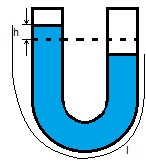
\includegraphics[height=30mm]{3_20.jpg}\\
	$phS \cdot \der{h}{t}{2} = \rho ghS + $\\
	$dF = mg B(x) dx \quad$ слой $dx$\\
	$\ddelta m \ddot x = \ddelta F$\\
	$\ddelta m = \rho x S \ddot x$\\
	$m \der{h}{t}{2} = \int\limits_{U - h}^{-U-h}\, dF = -2hg\rho S$\\
	$\cancel{\rho} \der{h}{t}{2} = -2 \cancel{\rho} ghS \Rightarrow \omega = \sqrt{\frac{2gS}{V}}$\\
	$T = \frac{2 \pi}{\omega} \quad T = \pi \sqrt{\frac{2V}{gS}}$\\
}

